

\documentclass[12pt]{article}
\usepackage{subfig}
\usepackage[english]{babel}
\usepackage[utf8x]{inputenc}
\usepackage[T1]{fontenc}
\usepackage{amsmath}
\usepackage{graphicx}
\usepackage{pstricks,pst-node}
\usepackage{stmaryrd}
\usepackage{gastex}
\usepackage{comment}
\usepackage{xcolor}
\usepackage{listings}
\usepackage{float}
\usepackage{url}





\catcode`\_=12

\definecolor{mGreen}{rgb}{0,0.6,0}
\definecolor{mGray}{rgb}{0.5,0.5,0.5}
\definecolor{mPurple}{rgb}{0.58,0,0.82}
\definecolor{backgroundColour}{rgb}{0.95,0.95,0.92}

\lstdefinestyle{CStyle}{
    backgroundcolor=\color{backgroundColour},   
    commentstyle=\color{mGreen},
    keywordstyle=\color{magenta},
    numberstyle=\tiny\color{mGray},
    stringstyle=\color{mPurple},
    basicstyle=\footnotesize,
    breakatwhitespace=false,         
    breaklines=true,                 
    captionpos=b,                    
    keepspaces=true,                 
    numbers=left,                    
    numbersep=5pt,                  
    showspaces=false,                
    showstringspaces=false,
    showtabs=false,                  
    tabsize=2,
    language=C
}




\usepackage[colorinlistoftodos]{todonotes}
\usepackage{wrapfig}

\begin{document}

\begin{titlepage}

\newcommand{\HRule}{\rule{\linewidth}{0.5mm}} % Defines a new command for the horizontal lines, change thickness here

\center % Center everything on the page
 
%----------------------------------------------------------------------------------------
%	HEADING SECTIONS
%----------------------------------------------------------------------------------------


\textsc{\Large Projet de recherche}\\[0.5cm] % Major heading such as course name
\textsc{\large "LU3IN013"}\\[0.5cm] % Minor heading such as course title

%----------------------------------------------------------------------------------------
%	TITLE SECTION
%----------------------------------------------------------------------------------------

\HRule \\[0.4cm]
{\huge \bfseries Système de vision temps réel pour drones}\\[0.4cm] % Title of your document
\HRule \\[1.5cm]
 
%----------------------------------------------------------------------------------------
%	AUTHOR SECTION
%----------------------------------------------------------------------------------------

\begin{minipage}{0.4\textwidth}
\begin{flushleft} \large
\emph{Equipe:}\\~\\

Johan-Luca \textsc{Rossi}\\
Qingyuan \textsc{Yao}\\
Lina \textsc{Saichi}\\
Mohamed \textsc{Meziane}\\
Melissa \textsc{Larbi}\\
Syrine \textsc{Marzougui}\\
% Your name
\end{flushleft}
\end{minipage}
~
\begin{minipage}{0.4\textwidth}
\begin{flushright} \large
\emph{Encadrants:} \\~\\
Fabrice \textsc{Kordon}\\ % Supervisor's Name
Lionel \textsc{Lacassagne}\\~\\~\\~\\~\\
\end{flushright}
\end{minipage}\\[2cm]

% If you don't want a supervisor, uncomment the two lines below and remove the section above
%\Large \emph{Author:}\\
%John \textsc{Smith}\\[3cm] % Your name

%----------------------------------------------------------------------------------------
%	DATE SECTION
%----------------------------------------------------------------------------------------

 % Date, change the \today to a set date if you want to be precise

%----------------------------------------------------------------------------------------
%	LOGO SECTION
%----------------------------------------------------------------------------------------

\includegraphics[scale=0.5]{logo.png}\\[1cm] % Include a department/university logo - this will require the graphicx package
 
%----------------------------------------------------------------------------------------

\vfill % Fill the rest of the page with whitespace

\end{titlepage}




%DEBUT DU DOC 


\renewcommand{\contentsname}{Sommaire}
\tableofcontents
\newpage

\section{Introduction}

Dans le cadre du projet de recherche, nous avons réalisé ce document qui présente notre compréhension des différents problèmes posés par celui-ci et des pistes de solutions que nous avons trouvées jusque-là. \\
Ce projet consiste à implémenter un programme qui permet à un drone (Parrot Bebop 2) de décoller et de s'orienter dans une pièce fermée (gymnase) pour trouver une cible (cf. figure 1) et atterrir devant et tout cela de manière autonome. Ce programme tournera sur une machine en liaison wifi avec le drone dans un premier temps, selon l'avancement du projet, il pourra être intéressant d'implémenter le programme directement sur la machine embarquée par le drone. \\On verra donc dans les sections qui suivent, comment nous avons défini l'architecture du projet et les grandes partie qui le constituent, et donc les différents objectifs, contraintes auxquelles chaque parties devra faire face et les protocoles mis en place jusque-là pour commencer à les résoudre.

\begin{figure}[H]
    \centering
    \subfloat[Format de la mire (cible)]{{\includegraphics[width=4cm]{mire.png} }}
    \qquad
    \subfloat[Le drone: Parrot Bebop 2]{{\includegraphics[width=5cm]{drone-parrot-bebop2-blanc.jpeg} }}
    \caption{Mire et drone}
    \label{fig:example}
\end{figure}




\section{Architecture du projet et étapes clés}

\paragraph*{Architecture:}
Dès le début, nous avons identifié trois aspects différents, mais tout aussi importants de ce projet. Il va donc se diviser en trois parties principales:
Une partie pilotage ayant pour but de contrôler le drone, d'apprendre à lui envoyer des instructions et à récupérer son flux vidéo, une partie imagerie de bas niveau devant développer des algorithmes de traitement d'images pour détecter la cible et enfin une partie imagerie de haut niveau qui elle, devra en fonction du positionnement de la cible émettre une décision sur les déplacements du drone.\\
Voici une version vulgaire de l'architecture qui décrit les taches reparties entre chaque partie:

\begin{figure}[H]
\centering
\includegraphics[height=10cm]{ArchiVulgaire.png}
\caption{Schéma d'architecture}
\end{figure}

\paragraph*{Étapes clés et scénarios:}
Nous avons fixé deux étapes importantes dans le développement de ce projet. Celles-ci correspondent à deux scénarios que le drone devra résoudre. 
\begin{itemize}
\item 
Scénario 1: Le drone démarre avec la mire en vue, il faudra alors qu'il arrive à se déplacer jusqu'à celle-ci et atterrir devant une fois assez proche.
\item 
Scénario 2: Le drone démarre, mais la cible n'est pas en vue, il devra alors la trouver et enfin appliquer le scénario 1. 
\end{itemize}

\section{Pilotage\label{pilotage}}

\subsection{Objectifs}
\paragraph*{Gérer la liaison avec le drone (réseau):}
Il faudra établir la connexion wifi avec le drone pour lui envoyer des instructions.
Il faudra aussi récupérer le flux vidéo pour l'imagerie de bas niveau.

\paragraph*{Comprendre le pilotage du drone:}
Il faudra dans un premier temps maîtriser les commandes de déplacements envoyées au drone, apprendre à "communiquer" avec celui-ci.
Dans un second temps, calibrer les commandes en corrélant la valeur des paramètres des commandes et le déplacement du drone. Enfin il faudra corréler les décisions de déplacement (cf.\ref{haut} Imagerie de Haut niveau) et l'amplitude des commandes à envoyer au drone une fois le calibrage réalisé.


\subsection{Contraintes}

\paragraph*{Contraintes de réseau:}
 On trouve les contraintes liées à la liaison avec le drone: latence de l'envoie des commandes ou stabilité de la connexion avec le drone. \\
Ces contraintes ont l'air jusque-là minimes, mais des tests seront quand même réalisés pour identifier leurs importances.

\paragraph*{Contraintes du mouvement:}
Le drone étant un système cyber-physique, on trouve d'abord les contraintes dynamiques (mouvement du drone) avec essentiellement : l'inertie du drone dans ses déplacements. On trouve une seconde moins importante: le souffle des hélices du drone sur lui-même a basse altitude.\\
L'importance et l'adaptation à ces contraintes seront clairement identifiées pendant le calibrage.



\subsection{Technologies utilisées}
\subsubsection{Contrôle du drone: Parrot SDK3}
 Le SDK \cite{SDK} va nous permettre de nous connecter, piloter et recevoir le flux vidéo du drone. Il est disponible en Java, C et Objective C, mais étant majoritairement écrit en C et pour éviter le multi-langages avec les autres parties, nous l'utiliseront uniquement en C. De plus, de nombreux outils ont déjà été développés avec le SDK pour le Bebop 1 et 2 en C.\\~\\
 Pour la compilation et l'exécution de programmes, le SDK utilise un système de build appelé Alchemy \cite{alchemy}, il permet de simplifier la gestion des makefiles, seul un makefile local et nécessaire par application, Alchemy permet de gérer toutes les dépendances générales, on verra dans la partie Prototypage et tests (cf.\ref{proto}) comment on a encore plus simplifié la compilation et l'exécution des programmes (cf.\ref{protor} scripts utiles). 
 
\subsubsection{Banc de tests: Parrot-Sphinx}
Parrot-Sphinx \cite{sphinx} est un outil de simulation initialement pensé pour couvrir les besoins des ingénieurs Parrot. La qualité de ce simulateur nous a permis et va nous permettre de réaliser des tests relativement précis sur les prototypes développés avant les tests sur le drone physique.\\
La manipulation du simulateur (connexion au drone...) est exactement la même que pour le vrai drone et dispose de fonctions intéressantes comme la capture du flux vidéo dans l'environnement du simulateur (qui lui-même est modifiable: ajout d'une cible ...) ce qui nous permettra de tester des programmes avancés avec détection de cible par exemple.

\begin{figure}[H]
\centering
\includegraphics[height=5cm]{world.jpg}
\caption{Le drone et la mire dans Sphinx}
\end{figure}

On va donc pouvoir réaliser des prototypes de programmes, les tester dans un premier temps sur Sphinx pour s'assurer de leur bon déroulement et de leur sécurité.
Ensuite on pourra les réaliser sur le drone physique. Cela nous permet donc de valider un protocole de test robuste.

Afin de créer un modèle 3D de la mire et de l'implémenter dans le monde simulé, des outils de création ont été utilisés. Nous sommes partis en recréer la mire en vecteurs dans Affinity Designer (similaire à Adobe Illustrator), ensuite le modèle 3D de la mire (.dae) a été créé dans Blender. Finalement, dans Gazebo, le logiciel sur lequel Sphinx est basé, nous avons réussi à convertir .dae à .sdf pour enfin insérer le modèle dans un monde (.world).


\subsection{Prototypage\label{proto}}
Les prototypes de programmes que nous avons et allons développer ont été basés sur l'exemple de programme BebopSample \cite{bebopsample} fourni par Parrot. Cet exemple permet de se connecter et de piloter le drone avec les touches du clavier. On a donc gardé l'essentiel de cet exemple pour développer la plupart des tests présentés plus bas.

\subsubsection{Commandes de déplacements}
Les commande de déplacement se présentent comme suit:\\~\\
\begin{minipage}{.5\linewidth}
\begin{itemize}
    \item Roll:Translation Gauche/Droite
    \item Pitch:Translation Avant/Arrière
    \item Yaw:Rotation Gauche/Droite
    \item Gaz:Translation Haut/Bas\\
\end{itemize}
\end{minipage}
\hfill
\begin{minipage}{.5\linewidth}
\centering
\includegraphics[width=.5\linewidth]{index.jpeg}
\end{minipage}
\\
Ces commandes sont définies selon les valeurs du pourcentage d'angle max (inclinaison du drone pour Roll,Pitch), de vitesse max (Rotation: Yaw /Translation: Gaz) et du temps pendant lesquelles elles sont réalisées. À ce stade, nous avons rendu compte qu'il est plus intéressant d'envoyer des commandes très courtes au drone étant donné qu'à chaque image que le drone capture, un traitement sera réalisé et une décision sera prise(cf. Imagerie et décision), l'impulsion durera le temps durant lequel le traitement suivant sera réalisé et stoppée à la commande suivante.

\subsubsection{Prototypes réalisés\label{protor}}
\paragraph*{Tests de déplacements:}
On a pu dans un premier temps, vérifier la bonne compréhension et le bon fonctionnement de notre protocole expérimental en réalisant des tests simples comme le décollage et l'atterrissage du drone ou encore le test de tous les déplacements possibles.
\paragraph*{Tests de calibration:}
Pour commencer à s'intéresser au comportement du drone avec de courtes impultions, nous avons réalisé un test de calibration qui permet de définir l'amplitude et la durée des impultions. On a pu réaliser l'expérience avec le drone physique et avec des marquages au sol, et donc corrélé ces paramètres et le déplacement du drone.\\
Nous avons aussi réalisé un test ayant uniquement pour but de corréler la taille de l'image de la cible sur la vidéo de la caméra du drone et la distance qui les séparent.

\paragraph*{Test de récupération du flux vidéo:}
Le BobopSample fourni par Parrot contient déjà le passage du flux à mplayer avec execlp() qui crée un fils pour lancer une commande bash. Nous sommes partis sur cette observation. En modifiant les paramètres de execlp(), le flux est passé à ffmpeg(cf. partie Imagerie de bas niveau) pour qu'il puisse générer les jpeg avec la fréquence d'images désirée. \\
Nous passerons le flux et la méthode de la récupération à la partie Imagerie de bas niveau.

\paragraph*{Scripts utiles (wifi et compilation):}

La procédure du pré-lancement qui consiste la connexion au wifi du drone avec mcli\cite{nmcli}, la compilation du code C (si elle n'est pas encore faite) avec Alchemy\cite{alchemy}, et le lancement de l'exécutable.


\section{Imagerie de bas niveau\label{bas}}
\subsection{Objectifs de la partie}
L'objectif de cette partie est d'analyser le flux vidéo capturé par la caméra du drone, et réaliser les deux premières étapes du traitement d'image : \\         
\textbf{Prétraitement : }opérations de
manipulation de l'image pour améliorer la
qualité, car il est impératif d'extraire la bonne information à bas niveau.
\textbf{Analyse : }suite d'opérations pour l'extraction
d'informations contenues dans une image. Dans ce projet, l'information qui nous intéresse est la présence ou non de la cible; et dans le cas favorable, sa position sur l'image.


\subsection{Contraintes}
\paragraph*{Temps de traitement:}
Le flux vidéo récupéré de la partie pilotage a une fréquence de 24 images/seconde. Il faudra traiter une image (traitement bas, moyen et haut niveau) en 1/24 secondes, ce qui fait en moyenne 42 millisecondes. Il s'agit donc d'optimiser le code au maximum pour avoir un temps de réponse <= 42ms.
\paragraph*{Nombre de données à traiter:}
Il s’agit dans cette partie de traiter les
données brutes issues de la caméra du drone. C’est le bloc qui traite le plus grand nombre de données (tous les pixels dans le cas du traitement
d’image).
\paragraph*{Contraintes liées au traitement d'image:}
L'environnement de test peut contenir des similitudes avec les quatre hirondelles de la mire. De ce fait, la détection de celle-ci peut paraître plus compliquée que prévu car on peut détecter d'autres objets outre que la mire qui lui ressemblent ( les cages du gymnase Jean Talbot).
Lors de nos essais , nous avons aussi remarqué qu'une hirondelle peut être considérée plusieurs fois comme un point d'intérêt.




\subsection{Description du  \textit{workflow}}
\label{section:Workflow}
 \begin{figure}[H]
\centering
\includegraphics[height=6cm]{workflowG.png}
\caption{Schéma représentatif des différentes entrées sorties de la partie imagerie bas niveau. }
\label{fig:WorkflowG}
\end{figure}


La partie relative à l'imagerie bas niveau est divisée en deux parties principales [Figure \ref{fig:WorkflowG}]. L'étape 1 concerne le traitement du flux vidéo que nous récupérerons de la partie pilotage. Nous allons le décomposer pour en récupérer des images. Celles-ci seront traitées au cours de la deuxième étape qui consiste à leur appliquer des algorithmes de traitement d'images ( détaillés dans la section ~\ref{section:Traitement}). L'objectif est de récupérer les coordonnées des quatre hirondelles de la mire [Figure \ref{fig:example}].
La partie imagerie haut niveau aura en entrée ces coordonnées.


\subsection{Outils et bibliothèques utilisées}
\subsubsection{Flux vidéo : FFMPEG}
FFMPEG \cite{FFMPEG} est un logiciel open source gratuit qui permet de traiter des flux multimédias. Il fournit une grande variété de formats pour les vidéos , audio, et images. On s'en sert pour traiter le flux vidéo du drone.\\ FFMPEG inclut plusieurs bibliothèques. Celles que nous avons utilisées sont : \textbf{libravcodec} qui fournit de nombreux décodeurs et encodeurs pour le flux vidéo, \textbf{libavutil} qui est une bibliothèque utilitaire qui nous fournit les structures de données, \textbf{libravformat} pour multiplexer et demultiplexer le flux et enfin \textbf{libswscale} pour les redimensionnements d'image.

\subsubsection{Images : OpenCV}
OpenCV \cite{OpenCV} est une bibliothèque graphique spécialisée dans le traitement d’images. Elle fournit des fonctions et algorithmes de traitement d'images accessibles à travers son API. Les modules utilisés dans ce projet sont:\\
\textbf{core} qui fournit les fonctionnalités de base. Cette bibliothèque permet de manipuler les structures de base, réaliser des opérations sur des matrices, dessiner sur des images...etc\\La deuxième bibliothèque utilisée est \textbf{highgui} : celle-ci contient un certain nombre de fonctions permettant de réaliser des interfaces graphiques très simples pour ouvrir , enregistrer et afficher des images et des flux vidéo.


\subsection{Traitement d'image}
\label{section:Traitement}

 \begin{figure}[H]
\centering
\includegraphics[height=7cm]{workflowI.png}
\caption{Schéma représentatif des différentes entrées sorties de la partie imagerie bas niveau en zoomant sur la partie traitement. }
\label{fig:WorkflowI}
\end{figure}

Ce schéma met en avant la deuxième étape du traitement du flux. Comme déjà mentionné dans la section~\ref{section:Workflow}, elle consiste à l'analyse d'images.
Nous pouvons en distinguer deux étapes successives : traitement bas et moyen niveau qui sont détaillées ci-dessous.

\subsubsection{Opérateur bas niveau }
Dans cette partie, nous allons récupérer l'image et y appliquer du traitement bas niveau afin d'améliorer sa qualité. \\
Par ailleurs, les images qu’on aura en entrée seront 
en couleurs, la première chose à faire sera de la transformer en image à
niveau de gris (m=8, le nombre de bits sur lesquels est codée la valeur
d’un niveau de gris). Elle prend ses valeurs dans l’ensemble \{0 .. 255\}, ou
le 0 et 255 correspondent respectivement au blanc et au noir, et les valeurs
intermédiaires correspondent aux différentes transitions entre les deux. Le
but de cette transformation est de minimiser la taille en mémoire que
prendra chaque image et pour nous faciliter ensuite la recherche de la mire.\\
Ensuite, nous allons ajuster le contraste de l'image en utilisant la méthode d'égalisation d'histogramme.


\subsubsection{Opérateur moyen niveau }
Une fois la qualité de l'image améliorée, nous allons commencer le traitement moyen niveau. Le but de cette partie est de trouver et retourner les coordonnées des centres des 4 hirondelles de la mire.\\
Afin de détecter les points d'intérêts, ce qu'on pourrait faire est d'utiliser une approche  à base de modèles : ces points seront identifiés dans l’image par mise en correspondance de leur intensité avec un modèle théorique des intensités, vu que nous connaissons déjà la couleur et la forme de la mire [Figure~\ref{fig:example}].\\

\subsection{Solutions possibles aux problèmes }
En ce qui concerne le traitement d'image, on va détecter plusieurs points d'intérêts, puis nous allons déterminer un ratio pour en choisir les quatre meilleurs.
Pour éviter qu'une hirondelle soit détectée plusieurs fois, nous allons réaliser de l'étalonnage sur les images selon les distances pour essayer de déterminer l'espacement minimum que deux hirondelles doivent respecter.


\section{Imagerie de haut niveau\label{haut}}
\subsection{Présentation et objectifs de la partie} 
Après avoir appliqué les différentes stratégies sur le flux des images dans la partie imagerie bas niveau qui ont permit d'extraire les cordonnées des hirondelles, il est temps d'en tirer un avantage. En effet dans cette partie on s'intéresse à l'estimation de la position du drone sur les axes x, y et z afin d'estimer une meilleure commande qui sera ensuite renvoyée à la partie pilotage, qui contre à elle, la traduira  en langage bas niveau pour piloter le drone comme le montre le figure \ref{les axes du drone}.\\ 

En terme algorithmique, cette partie prend en entrée l'estimation des cordonnées des hirondelles de la mire et renvoie en sortie l'estimation du déplacement à effectuer comme le montre la figure \ref{Architecture imagerie de haut niveau}.
\setlength{\unitlength}{1cm}
    \begin{figure}[h!]
    \centering
    \includegraphics[scale=0.7]{DRONE.PNG}
    \caption{\label{les axes du drone}les axes du drone}
    \end{figure}
\setlength{\unitlength}{1cm}
    \begin{figure}[h!]
    \centering
    \includegraphics[scale=0.7]{inout.png}
    \caption{\label{Architecture imagerie de haut niveau}Architecture imagerie de haut niveau}
    \end{figure}



\subsection{Une analyse technique du problème}
Lors de l'analyse profonde des tâches à réaliser dans cette partie on a identifié les différents problèmes qu'on aura à résoudre au fur et à mesure de l'avancement du projet dont on cite: 

\begin{itemize}
\item Estimer la position du drone sur les axes x, y et z en utilisant les informations reçues sur la position de la mire dans les images.
\item Estimer la profondeur entre le drone et la mire.
\item Gérer les cas de manque ou d'absence totale des informations sur la position de la mire dans les images. 
\item L'intervalle du temps maximal où on autorise le drone à rester inactif. Ce qui est traduit dans notre partie par le temps du traitement avant d'estimer le mouvement à réaliser. 
\end{itemize}


\subsection{Les solutions possibles pour résoudre ces problèmes }
Toutes les solutions qu'on va proposer dans la suite seront dans le cadre de l'utilisation du principe de la logique floue, c'est la méthode de résolution qu'on a adopté dans cette partie pour contrôler les mouvements du drone. \\
La logique floue\cite{LaLogiqueFloue}: c'est une méthode moderne de contrôle qui diffère de la logique classique. Elle était proposée par Zadeh en 1965. Elle nous permet d'exprimer différents niveaux pas seulement le 0 et le 1.\\
On a opté pour cette méthode par manque des précisons qu'on peut avoir sur la position et la profondeur du drone dans ses mouvements. Alors pour bien affronter ce problème l'utilisation de ce principe nous a paru comme une bonne solution déjà non gourmande en terme de ressource physique(mémoire), temps de traitement et aussi en terme d'informations pré-requises.

\subsubsection{Estimations de la position}
Avant de pouvoir estimer le mouvement à effectuer par le drone il est nécessaire d'identifier sa position pour cela on propose d'avoir des automates qui nous renseignent sur la position actuelle du drone sur les axes x, y et z.
Chaque état de ces automates est identifié à l'aide de la déformation que prend la mire sur les images comme c'est mentionné dans la figure \ref{forme de la mire}. \\

\setlength{\unitlength}{1cm}
    \begin{figure}[h!]
    \centering
    \includegraphics[scale=0.7]{ROTATION2.PNG}
    \caption{\label{forme de la mire}la forme de la mire}
    \end{figure}
     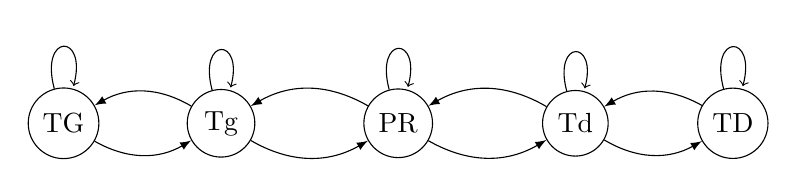
\begin{tikzpicture}
    \node[circle,draw=black](v1)at(3.5,0){TG};
    \node[circle,draw=black](v2)at(5.5,0){Tg};
    \node[circle,draw=black](v3)at(7.75,0){PR};
    \node[circle,draw=black](v4)at(10,0){Td};
    \node[circle,draw=black](v5)at(12,0){TD};
    \draw[>=latex,->] (v1) to[bend right] (v2);
    \draw[>=latex,->] (v2) to[bend right] (v1);
    \draw[>=latex,->] (v3) to[bend right] (v2);
    \draw[>=latex,->] (v2) to[bend right] (v3);
    \draw[>=latex,->] (v3) to[bend right] (v4);
    \draw[>=latex,->] (v4) to[bend right] (v3);
    \draw[>=latex,->] (v5) to[bend right] (v4);
    \draw[>=latex,->] (v4) to[bend right] (v5);
    \draw (v1) edge[loop above] node{$ $} (v1);
    \draw (v2) edge[loop above] node{$ $} (v2);     
    \draw (v3) edge[loop above] node{$ $} (v3);  
    \draw (v4) edge[loop above] node{$ $} (v4);  
    \draw (v5) edge[loop above] node{$ $} (v5);  
    \end{tikzpicture}\\
    
Cette figure nous montre les formes de la mire sur des images prises depuis différentes positions. On y voit clairement que quand l'axe du drone est perpendiculaire à celui de la mire, elle apparaît carrée dans les images mais quand le drone fait des rotations  gauche ou droite on voit une déformation de la forme de la mire. Plus la rotation est importante plus la déformation l'est aussi. 


Pour faire simple et sans effectuer des calculs complexes qui peuvent nous renseigner sur la position du drone on a choisi de se concentrer sur la forme de la mire car les images c'est tout ce qu'on a comme outils qui peuvent nous renseigner sur l'environnement externe du drone.

\subsubsection{Manque ou Absence des informations}
Comme on l'a mentionné un peu en haut, on peut ne pas avoir toutes les quatre cordonnées des hirondelles de la mire ou même aucune d'elles suite à un mouvement qui a sorti la mire du champ de vison de la caméra du drone ou suite à un facteur extérieur du mécanisme qui a caché la mire du drone. La solution qu'on propose pour résoudre ce problème est de stocker au moins la dernière estimation du mouvement transmis à la partie pilotage.\\

On propose cette solution car elle nous permet de remettre la mire dans le champ de vision du drone seulement en renvoyant l'inverse de l'estimation du mouvement précédemment transmis. Cela nous permet de gagner du temps et de la mémoire qui seront nécessaires pour toute autre méthode qui aura le même résultat. 

\subsubsection{Estimation de la profondeur}
La méthode pour déterminer la profondeur proposée dans la littérature est fondée sur l’utilisation de la stéréovision qui simplifie largement le problème du point de vue théorique, mais cette méthode est assez complexe au niveau pratique (deux caméras au minimum à gérer). Notre drone étant doté d'une seule caméra, on a adopté alors la méthode de calibrage \cite{Calibrage} pour estimer la profondeur de la mire. 
Cette méthode consiste en général à déterminer la relation mathématique existant entre les coordonnées des points 3D de la scène observée et les coordonnées 2D de leurs projections dans l'image.

\section{Conclusion}
À ce stade nous avons donc pu clairement poser les principaux objectifs et contraintes de ce projet, de mettre en place des protocoles qui semblent nous permettre de réaliser ces objectifs et de palier a une partie de ces contraintes. Évidemment, il reste des problèmes à résoudre et nous allons très sûrement en rencontrer de nouveaux au fur et à mesure de notre avancée.\\
Par l'intermédiaire d'un ordinateur faisant voler le drone et une caméra intégrée, on est arrivé à proposer des solutions de pilotage qui récupèrent le flux vidéo et qui contrôlent correctement le drone.
Nous sommes arrivés à décomposer le flux en images et à l'aide des algorithmes de traitement d'images, nous avons pu améliorer leur qualité et réussi à détecter les centres de la mire. En dernier lieu, nous avons trouvé des stratégies intéressantes de décision de déplacement du drone en fonction de l'estimation de la position et de la déformation de la mire dans les images.



\begin{thebibliography}{12}
\bibitem{sphinx} 
Parrot Sphinx: \path{https://developer.parrot.com/docs/sphinx/whatissphinx.html}

\bibitem{SDK}
Parrot SDK3:
\path{https://developer.parrot.com/docs/SDK3/general-information}

\bibitem{alchemy}
Alchemy:
\path{https://github.com/Parrot-Developers/alchemy}

\bibitem{bebopsample}
BebopSample:
\path{https://github.com/Parrot-Developers/Samples/blob/master/Unix/BebopSample/BebopSample.c}

\bibitem{nmcli}
nmcli:
\path{https://linux.die.net/man/1/nmcli}

\bibitem{FFMPEG}
FFMPEG:
\path{https://www.ffmpeg.org/}

\bibitem{OpenCV}
OpenCV:
\path{https://docs.opencv.org/4.1.1/d1/dfb/intro.html}

\bibitem{Calibrage}
Calibrage:
\path{http://www.optique-ingenieur.org/fr/cours/OPI_fr_M04_C01/co/Contenu94.html}
\bibitem{LaLogiqueFloue}
LaLogiqueFloue:
\path{https://www.techno-science.net/glossaire-definition/Logique-floue.html}


\iffalse
\bibitem{Commande référencée vision pour drones à decollages et atterrissages verticaux}
HAL : archive ouverte:
\path{https://hal.archives-ouvertes.fr/tel-01092388/document}
\fi

\bibitem{bebop}
Parrot Bebop 2:
\path{https://www.parrot.com/assets/s3fs-public/2019-01/parrotbebop2ledronetoutenun.pdf}
 

\end{thebibliography}



\end{document}